\chapter{Loss Function}
Una \textbf{funzione di costo} (o loss function) è un elemento fondamentale nel Deep Learning, perché misura \textit{quanto sia sbagliata la predizione di un modello rispetto ai valori reali}. L'obiettivo dell'apprendimento automatico è quello di minimizzare questa funzione, cosicché faccia previsioni più accurate. La misurazione delle funzioni di costo, risulta essere fondamentale per un criterio valutativo, inoltre permette di effetuarvi la Backpropagation nelle reti neurali.
\section{MSE Loss}
La funzione \texttt{nn.MSELoss()} calcola la Mean Squared Error (MSE) tra le predizioni e i valori target, questa tipologia di funzione di costo utilizza la L2 Norm:
\begin{equation}
L = \frac{1}{N} \sum_{i=1}^{N} (x_i - y_i)^2
\end{equation}
Essa risulta essere molto sensibile agli outlier, i valori marginali rispetto al fulcro dei dati, poiché gli errori vengono elevati al quadrato.
\section{L1 Loss}
La \texttt{nn.L1Loss()} invece misura il Mean Absolute Error (MAE), sempre tra le predizioni e i valori target, questa tipologia di funzione di costo utilizza la L1 Norm:
\begin{equation}
L = \frac{1}{N} \sum_{i=1}^{N} |x_i - y_i|
\end{equation}
Come possiamo immaginare rispetto alla precedente risulta essere più robusta alla presenza di outlier.
\section{L1 vs L2}
Ci si è chiesti pertanto, quale fra le due risulti essere migliore, alcune considerazioni si possono effettuare tramite delle visioni sperimentali. Si è mostrato come il con L2,i valori vengono distribuiti uniformemente, mentre con L1 i risultati sono netti. Pertanto riportando questa considerazione nei modelli di computer vision, si verifica sperimentalmente come L1 sia migliore quando ci sono delle immagini più "spigolose", diversamente otteniamo un risultato migliore con L2 in immagini che risultano essere più morbide nelle loro forme e nelle loro transizioni di colore (Figura~\ref{fig:l1l2diff}).

\begin{figure}
    \centering
    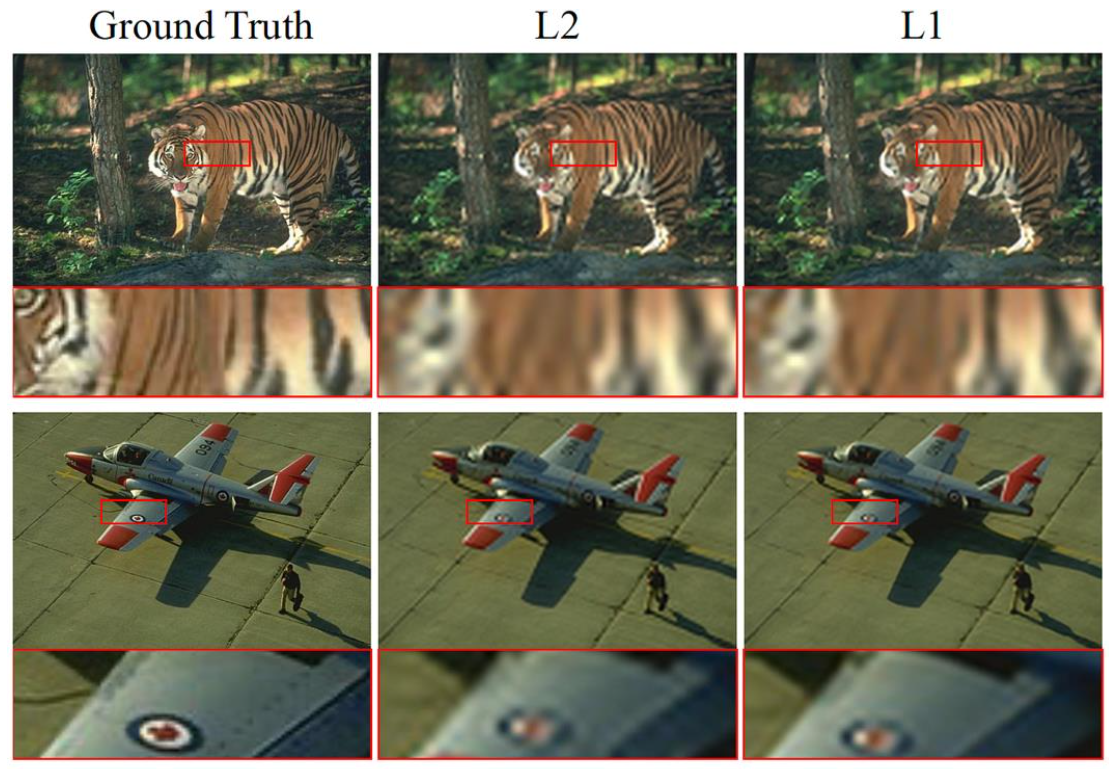
\includegraphics[width=0.75\linewidth]{figure/L1andL2.png}
    \caption{Utilizzando un modello di computer vision possiamo notare come è più accurata la norma 2 per figure meno spigolose, come quella della tigre, differentemente per l'immagine in cui vi è l'aereo la norma 1 è migliore poiché l'immagine risulta più spigolosa.}
    \label{fig:l1l2diff}
\end{figure}

\section{Smooth L1 Loss}
Notando come in alcune situazioni è meglio usare la norma 1 al posto della norma 2 e viceversa, si è strutturato un altro modello di Loss Function che le combina, la Smooth L1 Loss:
\begin{equation}
L(x, y) = \begin{cases} 
\frac{1}{2} (x - y)^2, & \text{se } |x - y| < 1 \\
|x - y| - \frac{1}{2}, & \text{altrimenti}
\end{cases}
\end{equation}

\section{Negative Log Likelihood Loss}
La Negative Log Likelihood Loss (NLL Loss) è una funzione di costo usata nei problemi di classificazione multi-classe. Questa Loss Function, prende i dati di output di un modello, solamente se espressi il probabilità logaritmica, quindi un vettore ottenuto tramite la funzione di attivazione $\operatorname{LogSoftMax}$, essa classificherà i vari dati, penalizzando in maniera ingente le predizioni sbagliate.

\begin{Esempio}
    Supponiamo di a vere un modello il quale ci fornisca 3 dati grezzi (logits) come di seguito:
    \begin{equation}
        z=[2.0\,,1.5\,,-1.0]
    \end{equation}
    Applicando la funzione $\operatorname{LogSoftMax}$ ottengo il seguente risultato:
    \begin{equation}
        \operatorname{LogSoftMax(z)} = [-0.42\,,-1.92\,,-3.42]
    \end{equation}
    Ora la NLL Loss determina la classe corretta e ne nega il segno, nel caso in cui la classe corretta risulti essere la prima ($0.42$) essa avra un costo, molto piccolo, pertanto è stata scelta la classe corretta, ma se accidentalmente il modello dovesse considerare la terza come classe corretta, avremo un costo elevato ($3.42$), questo ci fa comprendere come questa funzione di costo penalizzi fortemente le classificazioni effettuate con alta confidenza, in maniera errata, mentre favorisca quelle corrette.
\end{Esempio}
La formula della NLL Loss è la seguente:
\begin{equation}
    L = -\frac{1}{N}\sum^{N}_{i=1}\log P(y_i|x_i)
\end{equation}

\subsection{Problema delle classi sbilanciate}
Nel caso in cui avessimo un dataset sbilanciato, il modello tenderà a minimizzare la loss, trovando come soluzione, quella di predirre sempre la classe più frequente, producendo un esito falsato. La possibilità di aggiungere dei pesi per ogni classe, potrebbe essere un'idea:

\begin{equation}
    L = -\frac{1}{N}\sum^{N}_{i=1}w_{y_i}\log P(y_i|x_i)
\end{equation}

In questo modo, valorizzeremo la classe minoritaria, che altrimenti verrebbe schiacciata dall'altra allenando il nostro modello nella maniera scorretta. Questa soluzione però non è molto efficiente, come quella di avere un dataset bilanciato in partenza.

\section{Cross Entropy Loss}
La funzione \texttt{nn.CrossEntropyLoss()} combina \texttt{LogSoftmax} e \texttt{NLLLoss} in un'unica funzione ed è la più utilizzata nei problemi di classificazione multi-classe, essa viene definita come segue:
\begin{equation}
L = - \sum_{i=1}^{N} \sum_{j=1}^{C} y_{i,j} \log(\hat{y}_{i,j})
\end{equation}
dove:
\begin{itemize}
    \item $C$ è il numero di classi,
    \item $y_{i,j}$ è 1 se l'osservazione $i$ appartiene alla classe $j$, altrimenti è 0,
    \item $\hat{y}_{i,j}$ è la probabilità predetta per la classe $j$.
\end{itemize}
La Cross Entropy Loss, si comporta alla stessa maniera della Loss Function precedente, l'unica cosa che la diversifica è la dimensione implementativa, poiché la Cross Entropy accetta a differenza dell'altra direttamente i logits, per poi effettuarci la funzione di $\operatorname{LogSoftMax}$ di sua inziativa.

\section{Adaptive Log Softmax with Loss}
Quando si hanno problemi con molte classi, l'uso di una SoftMax standard può essere inefficiente, pertanto si è introdotta l'Adaptive Log Softmax With Loss (\texttt{nn.AdaptiveLogSoftmaxWithLoss()}). Questa funzione di perdita non fa altro che suddividere le classi in cluster, basati sulla loro frequenza. Essa adopera la funzione SoftMax per le classi più frequenti, mentre per quelle meno frequenti calcola in primis la probabilità del cluster e poi la probabilità del singolo elemento. In questo modo si suddividono le classi in maniera gerarchica, permettendo anche di effettuare delle riduzioni notevoli sul costo computazionale complessivo.

\section{Binary Cross Entropy Loss}
La Binary Cross Entropy Loss, è la versione binaria della Cross Entropy Loss, quindi nel momento in cui abbiamo solamente due classi nel nostro modello di classificazione, useremo la BCE Loss, la quale segue gli stessi principi della CE Loss, si introduce quindi la funzione \texttt{nn.BCELoss()}:
\begin{equation}
L = - \frac{1}{N} \sum_{i=1}^{N} -w_i\left[y_i \log({x}_i) + (1 - y_i) \log(1 - x_i) \right]
\end{equation}

\section{Kullback-Leibler Divergence Loss}
Nel momento in cui noi vogliamo misurare quanto la distribuzione target si discosti da quella predetta, possiamo utilizzare la Kullback Leibler Divergence Loss, basata sulla KL Divergence, una divergenza che misura quanto si discostano fra loro due distribuzioni di probabilità:
\begin{equation}
L = \sum_{i} P(i) \log \frac{P(i)}{Q(i)}
\end{equation}

\section{BCE Loss with Logits}
Un problema della BCE standard è che spesso per ottenere la sua probabilità usiamo la funzione sigmoide $\sigma(z)$, questo fattore porta a instabilità numerica. La \texttt{nn.BCEWithLogitsLoss()} incorpora direttamente la sigmoide nella perdita risolvendo il problema e rendendo tutto più stabile:
\begin{equation}
    L = - \frac{1}{N} \sum_{i=1}^{N} -\left[y_i \log(\sigma({x}_i)) + (1 - y_i) \log(1 - \sigma({x}_i) \right]
\end{equation}

\section{Hinge Embedding Loss}
Quando si lavora con problemi di similarità (es. metric learning), vogliamo una funzione di costo che enfatizzi la distanza tra esempi simili e dissimili. \texttt{nn.HingeEmbeddingLoss()} è utile in questi casi, lei insegna alla rete a tirare insieme le embedding di coppie simili e spingere lontano quelle diverse, finché la distanza supera una certa margin.

\section{Margin Ranking Loss}
Simile alla Hinge Loss, ma si usa in compiti di ranking dove dobbiamo garantire che un elemento più rilevante abbia punteggio più alto rispetto a un elemento meno rilevante, questo permette al sistema di ordinare al meglio ciò che desideriamo.
\begin{equation}
    L = \max(-y\,(x_1-x_2)+\text{margin},\,0) 
\end{equation}

Quì $x_1$ e $x_2$ sono gli output del modello per due esempi, mentre $y$ può assumere il valore $+1$ o $-1$, il primo se $x_1 > x_2$ e il secondo nel caso in cui $x_1 < x_2$ il margin invece è quanto vogliamo che i punteggi differiscano fra loro.

\section{Triplet Margin Loss}
Per migliorare la distinzione tra classi, \texttt{nn.TripletMarginLoss()} è ciò che viene utilizzato, questa confronta i valori con un'ancora (un valore fissato), con un esempio posiivo e uno negativo, dando la possibilità di espanderlo anche a più di due categorie:
\begin{equation}
L = \max(0, d(a, p) - d(a, n) + \text{margin})
\end{equation}

\section{Soft Margin Loss}
La Soft Margin Loss è una variante della Hinge Loss che introduce una penalità logistica per evitare margini rigidi:
\begin{equation}
L = \sum_{i=1}^{N} \log(1 + e^{-y_i x_i})
\end{equation}

Questa funzione di costo integra la funzione di SoftMax, alla logistica, aggiungendo un decadimento esponenziale alla funzione di costo.

\section{Cosine Embedding Loss}
Giungiamo ora all'ultima funzione di costo considerata in questa analisi. Immaginiamo di avere un insieme di frasi e di voler costruire un modello capace di riconoscere quando due frasi esprimono lo stesso significato, anche se formulate in modo diverso. In altre parole, vogliamo che frasi semanticamente simili vengano rappresentate da vettori vicini nello spazio latente, mentre frasi con significati differenti risultino più distanti.
\begin{figure}[h]
    \centering
    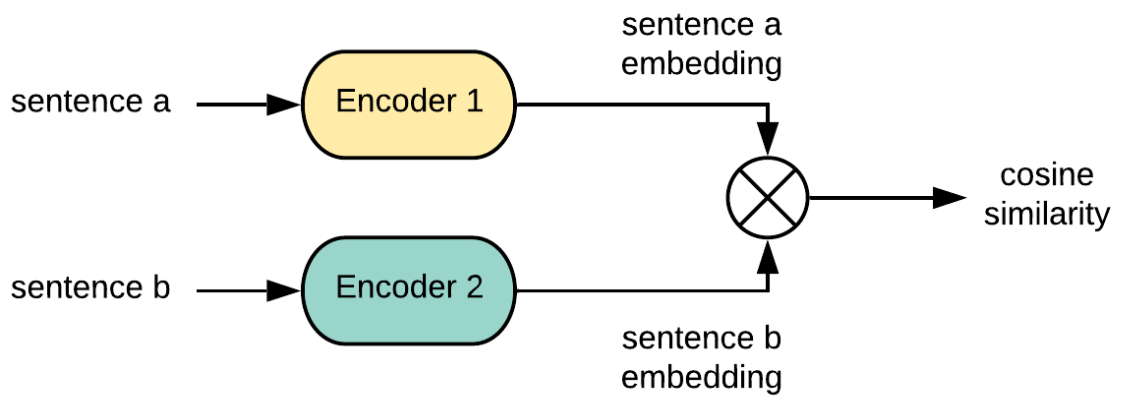
\includegraphics[width=0.75\linewidth]{figure/CosineSim.png}
    \caption{Rappresentazione di come vorrei siano trattate due frasi per determinarne la loro similarità.}
    \label{fig:coSim}
\end{figure}

Naturalmente, due frasi diverse, anche se trattano lo stesso argomento, tenderanno ad occupare posizioni diverse nello spazio delle embedding. Tuttavia, se il nostro obiettivo è misurare la somiglianza semantica, desideriamo che tali rappresentazioni siano quanto più possibile allineate, senza però perdere la ricchezza del linguaggio dovuta a tono, stile, gergo o espressività. Per quantificare la somiglianza tra due vettori di embedding si utilizza la \textbf{Cosine Similarity}, la quale misura il coseno dell’angolo compreso tra i due vettori:
\[
\cos(x_1, x_2) = \frac{x_1 \cdot x_2}{\|x_1\| \|x_2\|}
\]
Quando i due vettori sono perfettamente allineati, il coseno vale 1; quando sono ortogonali, vale 0; e quando puntano in direzioni opposte, vale -1.

\begin{Osservazione}
    Due vettori completamente diversi tendono ad essere ortogonali, indicando l’assenza di correlazione tra le loro direzioni nello spazio delle embedding.
\end{Osservazione}

La \texttt{nn.CosineEmbeddingLoss()} di \textit{PyTorch} sfrutta questa misura per addestrare modelli che devono apprendere relazioni di similarità o dissimilarità tra coppie di vettori. La sua formulazione è la seguente:
\begin{equation}
L = 
\begin{cases} 
1 - \cos(x_1, x_2), & \text{se } y = 1 \ (\text{coppie simili}) \\
\max(0, \cos(x_1, x_2) - \text{margin}), & \text{se } y = -1 \ (\text{coppie diverse})
\end{cases}
\end{equation}

Questa funzione di costo incoraggia i vettori appartenenti a coppie simili a essere orientati nella stessa direzione (coseno vicino a 1), e quelli di coppie dissimili ad avere un coseno più basso, ovvero a essere separati da un angolo ampio.  